% *********************** Це є Розділ 1 ************************************

 \markright{\underline {\it Розділ 1. Постановка задачі}}

 \setcounter{chapter}{0}
 \chapter{Моделювання фізично правильної взаємодії світла }

 
 \par У цьому розділі приведено визначенно основних терміні та визначенно основні проблеми, пов'язані з моделюванням фізично правильної взаємодії світла з 
      об'єктами в комп'ютерній графіці. 

 \section{Людське сприйняття зображень}
  \setcounter{equation}{0}
 \setcounter{theorem}{0}

 \par Перед тим як вдаватись до деталей моделювання фізично правильної взаємодії світла з об'єктами, важливо розглянути, 
 яким чином людське оке сприймає світло та як мозок формує зображення.
 \par Світло - це квантова елетромагнітна хвиля, швидкість якої рівна \\ $299\,792\,458\,\text{m/s}$. Видимий спектр світла знаходиться між 
 380 та 780 наномет\-рами рис. \ref{fig:LightSpectrum}. Видимо світло яке є монохромним відповідає деякему кольору спектру. Зазвичай джерела світла випромінюють 
 світло в широкому діапазоні довжин хвиль. Наприклад денне світло є суперпозицією деякого діапазону хвиль рис. \ref{fig:LightSuper}.
Спостерігати ми це можемо під час веселки, коли світло проходить через краплі води, розкладаючись на спектр кольорів.

 \begin{figure}[h]
  \centering
  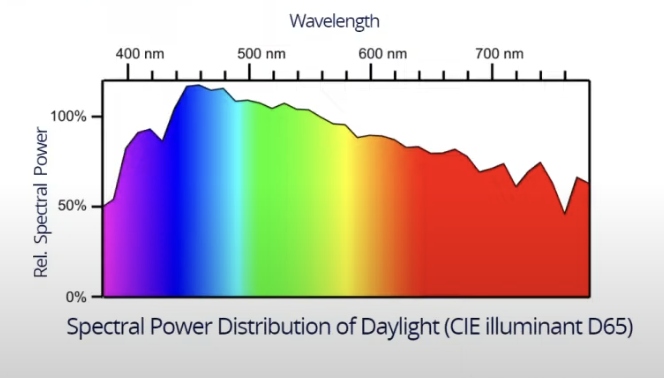
\includegraphics[scale=1]{Pictures/LightSuper.png}
  \caption{Спектральний розподіл енергії денного світла}
  \label{fig:LightSuper}
\end{figure}

\begin{figure}[h]
\centering
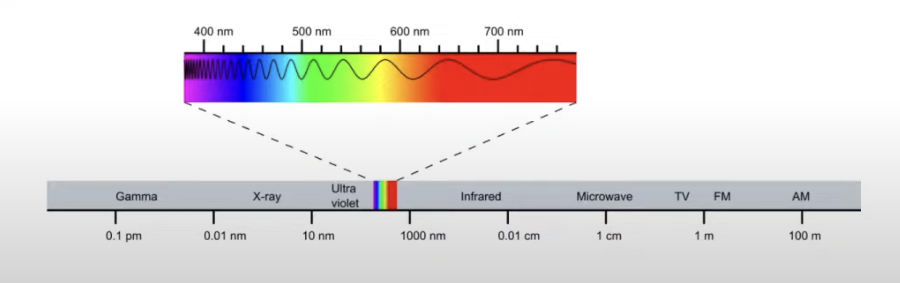
\includegraphics[scale=1]{Pictures/LightSpec.png}
\caption{Видимий спект світла}
\label{fig:LightSpectrum}
\end{figure}

  \par Світло також взаємодіє з навколишніми об'єктами. Припустимо, що світло випромінюється деяким джерелом в однорідних речовинах, наприклад повітрі
  світло рухається по прямій, деякі промені світла можуть попасти одразу в людське око, інші ж потрапляють на деякі об'єкти, які в свою чергу поглинають, відбивають або
  пропускають фотони світла. Відповідно до цього, ми можемо спостерігати різні кольори об'єктів, які залежать від того, які довжини хвиль світла вони відбивають.
  Те світло яке потрапляє в око людини, проходить через рогівку, кришталик та склоподібне тіло, де воно фокусуються на сітківці ока. Сітківка містить фоторецептори, 
  які реагують на світло і перетворюють його в електричні сигнали, що надсилаються до мозку. Мозок обробляє ці сигнали і формує зображення, яке ми сприймаємо.

 \begin{figure}[h]
  \centering
  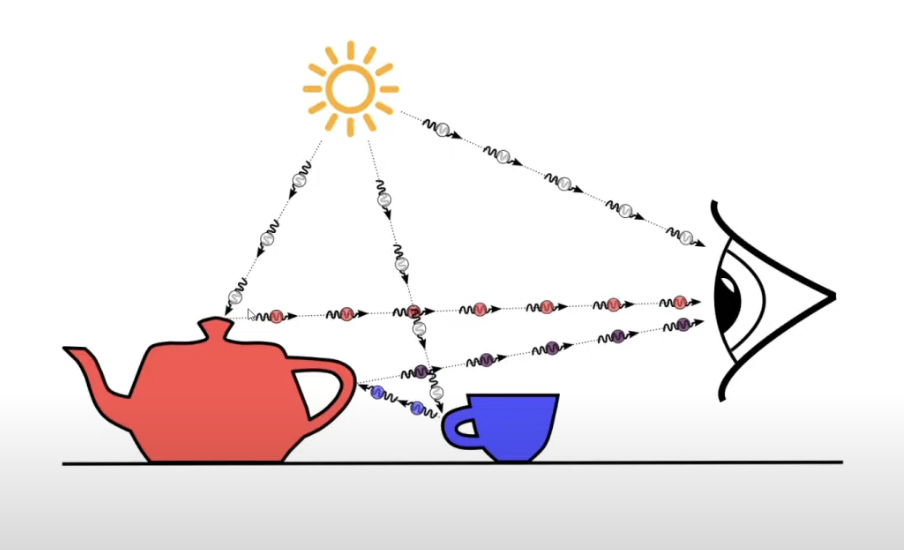
\includegraphics[scale=1]{Pictures/LightPath.png}
  \caption{Шлях світла від джерела до ока людини}
  \label{fig:LightPath}
\end{figure}

\par
Загалом у людини існують дві основні системи фоточутливих рецепторів, що забезпечують зорове сприйняття:
\begin{enumerate}
\item \textbf{Палички} — фоторецептори, які мають високу чутливість до інтенсивності світла та забезпечують зір при слабкому освітленні 
(скотопічний зір). Вони не розрізняють кольори.
\item \textbf{Колбочки} — рецептори, відповідальні за кольоровий (фотопічний) зір. Вони чутливі до різних діапазонів довжин хвиль електромагнітного 
випромінювання. Існує три типи колбочок рис. \ref{fig:LightRecept}:
\begin{enumerate}
    \item \textbf{L-колбочки} (Long) — реагують на довгі довжини хвиль (приблизно 560–580 нм), що відповідає червоному діапазону спектра.
    \item \textbf{M-колбочки} (Medium) — сприймають середні довжини хвиль (приблизно 530 нм), асоційовані із зеленим кольором.
    \item \textbf{S-колбочки} (Short) — чутливі до коротких довжин хвиль (приблизно 420–440 нм), які відповідають синьому кольору.
\end{enumerate}
\end{enumerate}

 \begin{figure}[h]
  \centering
  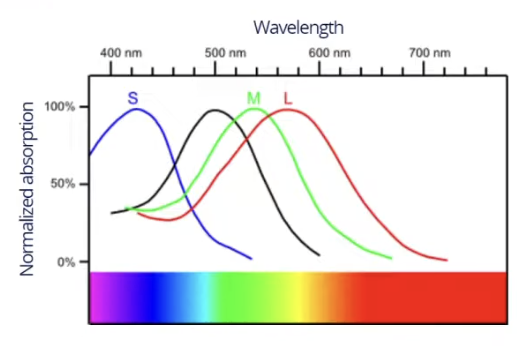
\includegraphics[scale=1]{Pictures/LightRecept.png}
  \caption{Людські колбочки та діапазон їх чутливості}
  \label{fig:LightRecept}
\end{figure}

Через те, що людське око має лише три типи колбочок, людське око не може сприймати реальний спектральний розподіл енергії світла,
завдяки цьому око можна обманювати, і різні спектрані розподіли енергії світла можуть сприйматись як однакові кольори. Саме через це, в комп'ютерній графіці
застосовується RGB кольорова модель, де R-red(червоний) G-green(зелений) B-blue(синій). Змішуючи ці три кольори в різних пропорціях, можна отримати 
більшість кольорів, які сприймаються людським оком рис \ref{fig:RGB}. Прямий фізичний зв'язок між спектральним розподілом енергії світла та RGB описано в \cite{Ch0} та \cite{Ch1}.
Більшість сучасних моніторів та екранів використовують sRGB кольорову модель для відображення зображень, але для фізично правильного рендерингу треба працювати в 
лінійному спектрі, для цього застосовується так звана \textit{гама корекція}, яка дозволяє перетворити кольори з sRGB в лінійний спектр \cite{Ch2}.
Основна ідея, яку слід засвоїти, полягає в тому, що немає потреби симулювати транспортування світла для кожної довжини хвилі окремо. Для більшості практичних застосувань 
достатньо розраховувати перентранспортуванняесення світла для трьох основних кольорів. Це значно спрощує обчислення та робить задачі 
рендерингу обчислювально ефективнішими.

\begin{figure}[h]
  \centering
  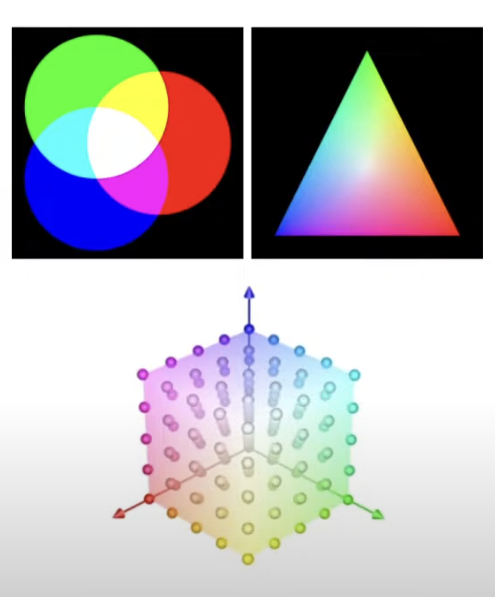
\includegraphics[scale=1]{Pictures/RGB.png}
  \caption{RGB кольорова модель}
  \label{fig:RGB}
\end{figure}

 \section{Визначення рівняння Рендерингу}
   \setcounter{equation}{0}
 \setcounter{theorem}{0}

 \subsection{Радіометричні величини}

Перш ніж дати визначення рівнянню рендерингу, варто розглянути деякі основні фізичні величини, які в ньому зустрічаються. Одним із базових понять є \textit{тілесний кут}.

\par
У школі ми вивчали поняття кута у двовимірному просторі. Щоб визначити, який кут охоплює об’єкт з певної точки спостереження, уявімо коло з центром у цій точці та проектуємо об’єкт на коло. Кут визначається як відношення довжини дуги $s$ до радіуса $r$:
\[
\theta = \frac{s}{r}
\]
Оскільки кут є безрозмірною величиною, його вимірюють у радіанах. 
\par
У тривимірному просторі аналогом звичайного кута є \textit{тілесний кут} (англ. \textit{solid angle}). Щоб визначити тілесний кут, який охоплює об’єкт з певної точки, розмістимо у цій точці центр уявної сфери та проектуємо об’єкт на її поверхню. Тілесний кут визначається як відношення площі проєкції $s$ до квадрата радіуса сфери:
\[
\omega = \frac{s}{r^2}
\]
Це також безрозмірна величина, яку вимірюють у \textit{стеррадіанах (sr)}. Повна сфера має тілесний кут $4\pi$ стеррадіан.

\par
Для обчислення тілесного кута, що покриває певну область, його розбивають на нескінченно малі елементи $d\omega$ і інтегрують по всій області:
\[
\omega = \int d\omega
\]

\par
Зручним способом параметризації є сферичні координати, які задаються двома кутами: полярним кутом $\theta$ (від $0$ до $\pi$) та азимутальним кутом $\phi$ (від $0$ до $2\pi$). Нескінченно мала ділянка тілесного кута виражається через поверхневий елемент $ds$:
\[
d\omega = \frac{ds}{r^2}
\]
Припускаючи, що радіус $r = 1$, обчислимо $ds$ як площу елемента поверхні сфери:
\[
ds = \sin{\theta} \, d\theta \, d\phi
\]
Таким чином, фінальна формула для нескінченно малої ділянки тілесного кута набуває вигляду:
\[
d\omega = \sin{\theta} \, d\theta \, d\phi
\]

А загальна формула для тілесного кута, що охоплює певну область на сфері, виглядає так:
\bql{eq:SolidAngle}
\omega = \int_0^{2\pi} \int_0^{\pi} \sin{\theta} \, d\theta \, d\phi
\eq

\paragraph{Потік випромінювання (Radiant Flux).}
Потік випромінювання, або \textit{radiant flux}~$\Phi$, — це енергія електромагнітного випромінювання, що передається в одиницю часу:
\[
\Phi = \frac{dQ}{dt}
\]
де $Q$ — енергія, $t$ — час. Одиниця вимірювання — ват (Вт), тобто джоуль на секунду (Дж/с).

Кожен фотон несе енергію
\[
E = \frac{hc}{\lambda}
\]
де $h$ — стала Планка, $c$ — швидкість світла, $\lambda$ — довжина хвилі.

Таким чином, потік випромінювання можна інтерпретувати як сумарну енергію фотонів, що випромінюються джерелом світла за одиницю часу. У графіці $\Phi$ 
використовується для опису загального випромінювання точкового джерела.

\paragraph{Інтенсивність випромінювання (Radiant Intensity).}
Інтенсивність випромінювання $I$ — це потік випромінювання на одиницю тілесного кута:
\[
I = \frac{d\Phi}{d\omega}
\]
Одиниця вимірювання — Вт/ср (ват на стеррадіан). Ця величина використовується, коли джерело випромінює нерівномірно в різних напрямках, як, наприклад, 
у випадку прожектора. Для точкового джерела, що випромінює рівномірно у всіх напрямках:
\[
I = \frac{\Phi}{4\pi}
\]

\paragraph{Опроміненість (Irradiance).}
Опроміненість $E$ — це потік випромінювання, що потрапляє на одиницю площі поверхні:
\[
E = \frac{d\Phi}{dA}
\]
Одиниця — Вт/м$^2$. Потік може надходити з усіх напрямків півсфери над поверхнею. Для нескінченно малої ділянки $dA$, яку 
освітлює точкове джерело, враховується тілесний кут $d\omega$, під яким джерело бачиться з цієї ділянки. Якщо $\theta$ — кут між нормаллю до 
поверхні та напрямком на джерело, то проєкція враховується через множник $\cos{\theta}$:

\[
E = \frac{I \cdot \cos{\theta}}{r^2}
\]

де $r$ — відстань до джерела.

Оскільки $I = \frac{\Phi}{4\pi}$, то для точкового джерела маємо:
\[
E = \frac{\Phi \cdot \cos{\theta}}{4\pi r^2}
\]

Це показує, що опроміненість спадає з квадратом відстані та залежить від кута падіння світла.

\paragraph{Енергетична яскравість (Radiance).}
Енергетична яскравість $L$ визначається як потік випромінювання, що проходить через одиницю площі в певному напрямку, на одиницю тілесного кута:
\[
L = \frac{d^2\Phi}{dA_{\perp} \, d\omega}
\]
де $dA_{\perp} = \cos{\theta} \, dA$ — проєкція площі в напрямку потоку. Одиниця — Вт/(м$^2$·ср).
Ця величина не залежить від відстані до джерела, адже при зменшенні відстані тілесний кут збільшується, але площа яка спостерігається - зменшується.
Спостергіти це явище ми можемо на прикладі стіни, змінючи відстань до неї, ми можемо спостерігати що яскравість стіни не змінюється.

\paragraph{Зв'язок між опроміненістю та енергетичною яскравістю.}
Опроміненість можна визначити через інтегрування енергетичної яскравості по всій півсфері $\Omega_h$ напрямків над поверхнею:
\bql{eq:RadianceToIrradiance}
E = \int_{\Omega_h} L(\omega) \cos{\theta} \, d\omega
\eq

\subsection{Рівняння рендерингу}
Рівняння рендерингу описує, як світло взаємодіє з поверхнями об'єктів і як це впливає на зображення, яке ми бачимо. Воно базується на фізичних принципах 
передачі світла та його взаємодії з матеріалами.
\bql{eq:RenderingEquation}
  L_o(\mathbf{v}) = L_e(\mathbf{v}) + \int_{\Omega_h} f_r(\mathbf{v},\mathbf{l} ) L_i(\mathbf{l}) \cos{\theta} d\omega
\eq

де: $L_o(\mathbf{v})$ — вихідна енергетична яскравість у напрямку $\mathbf{v}$, $L_e(\mathbf{v})$ — енергетична яскравість, що випромінюється поверхнею в напрямку $\mathbf{v}$,
$f_r(\mathbf{v},\mathbf{l})$ — \textit{Двопроменева функція розподілу відбивної здатності}(BRDF), що описує, як світло знапрямком $\mathbf{l}$ відбивається від 
поверхні в напрямок $\mathbf{v}$, $L_i(\mathbf{l})$ — вхідна енергетична яскравість у напрямк)у $\mathbf{l}$, 
$\theta$ — кут між нормаллю до поверхні та напрямком на джерело світла, $d\omega$ — тілесний кут.\\
Якщо придивитися уважно, то можна побачити, що рівняння рендерингу містить в собі рівняння для опроміненості \eref{eq:RadianceToIrradiance}.
\paragraph{Складність обчислення рівняння освітлення.}

Інтегрування по всій півсфері напрямків~$\Omega_h$ означає врахування всіх можливих напрямків поширення світла, яке може впливати на задану точку поверхні.
 Це робить рівняння освітлення обчислювально складним, адже для кожної точки сцени потрібно проінтегрувати внесок світла з усіх напрямків півсфери, орієнтованої 
 відносно нормалі до поверхні.

Кожен об’єкт у сцені сам по собі є джерелом випромінювання, тобто володіє певною вихідною енергетичною яскравістю в довільному напрямку~$\mathbf{v}$. Взаємне 
освітлення між об’єктами створює глобальну взаємозалежність, де світло, відбите від однієї поверхні, може впливати на інші поверхні, і так далі — потенційно нескінченну
 кількість разів.

Складність посилюється тим, що будь-яка поверхня є неперервною\footnote{Поверхня та кількість світлових променів у сцені є скінченними, проте їхня кількість настільки велика, 
що варто вважати їх нескінченними та неперервними} множиною точок, а з кожної точки в нескінченну кількість напрямків можуть надходити фотони. На 
мікроскопічному рівні поверхні не ідеально гладкі: вони можуть мати шорсткості, мікрогеометрію, відмінні оптичні властивості (наприклад, металічність, діелектричність,
 шорсткість тощо), що впливають на спосіб взаємодії зі світлом.

Оскільки світло може багаторазово відбиватися між поверхнями перед тим, як потрапити в камеру або око спостерігача, точне симулювання всіх траєкторій кожного 
фотона є обчислювально недосяжним\footnote{Існують методи, такі як Ray Tracing та Path Tracing, які симулюють поведінку світла, але лише для скінченної кількості променів, та
малої кількість відбитів світла від поверхонь} завданням для сучасних комп’ютерів.

У зв’язку з цим, замість точного моделювання всіх траєкторій, у комп’ютерній графіці застосовуються стохастичні методи, які описують розповсюдження світла у вигляді
 ймовірнісного процесу. Зокрема, розглядається ймовірність того, що промінь світла з певного напрямку~$\mathbf{l}$, взаємодіючи з поверхнею з відомими матеріальними 
 властивостями, буде відбитий в інший напрямок або поглинутий. Саме BRDF функція дозволяє моделювати цю ймовірність, і давати загальне уявлення про те, як світло
взаємодіє з поверхнею.\\
Варто зауважити, що такий підхид не дає точного рішення рівняння рендерингу, але дозволяє отримати
достатньо реалістичні результати за розумний час. У комбінації з іншими методами, такими як трасування променів, глобальне освітлення та інші,
можна досягти високої якості зображень, які виглядають фізично коректно, хоча і не є абсолютно точними.



